\documentclass[english]{beamer}\usepackage[]{graphicx}\usepackage[]{color}
%% maxwidth is the original width if it is less than linewidth
%% otherwise use linewidth (to make sure the graphics do not exceed the margin)
\makeatletter
\def\maxwidth{ %
  \ifdim\Gin@nat@width>\linewidth
    \linewidth
  \else
    \Gin@nat@width
  \fi
}
\makeatother

\definecolor{fgcolor}{rgb}{0.345, 0.345, 0.345}
\newcommand{\hlnum}[1]{\textcolor[rgb]{0.686,0.059,0.569}{#1}}%
\newcommand{\hlstr}[1]{\textcolor[rgb]{0.192,0.494,0.8}{#1}}%
\newcommand{\hlcom}[1]{\textcolor[rgb]{0.678,0.584,0.686}{\textit{#1}}}%
\newcommand{\hlopt}[1]{\textcolor[rgb]{0,0,0}{#1}}%
\newcommand{\hlstd}[1]{\textcolor[rgb]{0.345,0.345,0.345}{#1}}%
\newcommand{\hlkwa}[1]{\textcolor[rgb]{0.161,0.373,0.58}{\textbf{#1}}}%
\newcommand{\hlkwb}[1]{\textcolor[rgb]{0.69,0.353,0.396}{#1}}%
\newcommand{\hlkwc}[1]{\textcolor[rgb]{0.333,0.667,0.333}{#1}}%
\newcommand{\hlkwd}[1]{\textcolor[rgb]{0.737,0.353,0.396}{\textbf{#1}}}%
\let\hlipl\hlkwb

\usepackage{framed}
\makeatletter
\newenvironment{kframe}{%
 \def\at@end@of@kframe{}%
 \ifinner\ifhmode%
  \def\at@end@of@kframe{\end{minipage}}%
  \begin{minipage}{\columnwidth}%
 \fi\fi%
 \def\FrameCommand##1{\hskip\@totalleftmargin \hskip-\fboxsep
 \colorbox{shadecolor}{##1}\hskip-\fboxsep
     % There is no \\@totalrightmargin, so:
     \hskip-\linewidth \hskip-\@totalleftmargin \hskip\columnwidth}%
 \MakeFramed {\advance\hsize-\width
   \@totalleftmargin\z@ \linewidth\hsize
   \@setminipage}}%
 {\par\unskip\endMakeFramed%
 \at@end@of@kframe}
\makeatother

\definecolor{shadecolor}{rgb}{.97, .97, .97}
\definecolor{messagecolor}{rgb}{0, 0, 0}
\definecolor{warningcolor}{rgb}{1, 0, 1}
\definecolor{errorcolor}{rgb}{1, 0, 0}
\newenvironment{knitrout}{}{} % an empty environment to be redefined in TeX

\usepackage{alltt}
%% The most common packages are already included in:
\usetheme{biostat}
%%%%%%%%%%%%%%%%%%%%%%%%%%%%%%%%%%%%%%%%%%%%%%%%%%%%%%%% 
\usepackage{amsmath,amsfonts,tikz, amssymb}
\usetikzlibrary{trees}

%% Header data: (adjust to your needs:
\def\uzhunit{Biostatistics}             %% if (not) needed comment/uncomment
%\def\uzhunitext{STA480}

\title{Publication Bias in Meta-Analysis}%[Publication Bias]
%% Optional Argument in [Brackets]: Short Title for Footline

%% The following are all optional, simply comment them
%\subtitle{Publication Bias in the Cochrane Libary}
%\institute{Biostatistics Journal Club}  %% optional
\author{Giuachin Kreiliger}
%\date{\today}
%%%%%%%%%%%%%%%%%%%%%%%%%%%%%%%%%%%%%%%%%%%%%%%%%%%%%%%% 




%%%%%%%%%%%%%%%%%%%%%%%%%%%%%%%%%%%%%%%%%%%%%%%%%%%%%%%%
\IfFileExists{upquote.sty}{\usepackage{upquote}}{}
\begin{document}
\maketitle
%%%%%%%%%%%%%%%%%%%%%%%%%%%%%%%%%%%%%%%%%%%%%%%%%%%%%%%% 

% \begin{frame}{Evidence Synthesis}
% Summarise evidence over fields and studies
% 
% Quantitatively by meta-analysis
% 
% \end{frame}

\begin{frame}{Publication Bias}
Studies with large effects are more likely to be published

Incentives for bad research practices ($p$-hacking...)
\end{frame}

\begin{frame}{Meta-Analysis}
Aim to summarize evidence \& reach conclusions

classical meta-analyses rely on random sample assumption
\end{frame}

\begin{frame}{Fixed Effects Meta-Analysis}
Study $i$ of $n$ studies, effects $\theta_i$ and variances $v_i$, s.e. $s_i$

Fixed effects estimate: weighted mean with $w_i = 1/\hat{v_i}$: 

\begin{align}
\theta_f &= \frac{\sum_{i = 1}^n w_{i}\theta_i}{\sum_{i = 1}^n w_i} \nonumber \\ 
\textrm{se}(\theta_f) &= \frac{1}{\sqrt{\sum_{i = 1}^n w_i}} \nonumber
\end{align}
\end{frame}

\begin{frame}{Random Effects Meta-Analysis}
Let $\hat{\theta_i}|\theta_i \sim N(\theta_i, v_i) 
\theta_i \sim N(\theta, \tau^2)$

Random effects estimate: weigthed mean of $\hat{\theta_i}$ with weights $w_i = 1/(\hat{v_i} + \tau^2)$
\end{frame}

\begin{frame}{Evidence Based Medicine}
Likely to base decisions on over-optimistic findings

Direct consequences: patient harm and unnecessary research
\end{frame}


\begin{frame}{Cochrane Organisation}
Aim: summarise findings in primary clinical research and health care

Provide peer-reviewed, systematic reviews

Public access (for some countries)
\end{frame}

\begin{frame}{Research Question}
Quantify the abundance and impact of publication bias in the Cochrane Library
\end{frame}


\begin{frame}{Cochrane Library Dataset}
5,016 systematic reviews with studies published until 2018.

52,995 studies.

463,820 study results.
\end{frame}


\begin{frame}[fragile]{Review Example: Binary Outcome}
Barbiturate efficacy for head injury treatment
\vspace{-5mm}
% latex table generated in R 3.5.1 by xtable 1.8-3 package
% Mon May 20 22:21:48 2019
\begin{table}[ht]
\centering
\begingroup\tiny
\begin{tabular}{lllrrrr}
  \hline
Study & Comparison & Outcome & Events & Total & Events\_c & Total\_c \\ 
  \hline
Bohn 1989 & Barbiturate vs no b & Death at the end of & 11 & 41 & 11 & 41 \\ 
  Bohn 1989 & Barbiturate vs no b & Death or severe dis & 18 & 41 & 13 & 41 \\ 
  Eisenberg 1988 & Barbiturate vs no b & Uncontrolled ICP du & 25 & 37 & 30 & 36 \\ 
  Eisenberg 1988 & Barbiturate vs no b & Hypotension during  & 23 & 37 & 18 & 36 \\ 
  Perez-Barcena 2008 & Pentobarbital vs Th & Death at the end of & 16 & 21 & 9 & 21 \\ 
  Perez-Barcena 2008 & Pentobarbital vs Th & Death or severe dis & 17 & 21 & 13 & 21 \\ 
  Perez-Barcena 2008 & Pentobarbital vs Th & Uncontrolled ICP du & 18 & 22 & 11 & 22 \\ 
  Perez-Barcena 2008 & Pentobarbital vs Th & Hypotension during  & 20 & 22 & 21 & 22 \\ 
  Schwartz 1984 & Barbiturate vs Mann & Death at the end of & 6 & 15 & 7 & 14 \\ 
  Schwartz 1984 & Barbiturate vs Mann & Uncontrolled ICP du & 19 & 28 & 12 & 31 \\ 
  Ward 1985 & Barbiturate vs no b & Mean ICP during tre & 0 & 27 & 0 & 26 \\ 
  Ward 1985 & Barbiturate vs no b & Mean arterial press & 0 & 27 & 0 & 26 \\ 
  Ward 1985 & Barbiturate vs no b & Mean body temperatu & 0 & 27 & 0 & 26 \\ 
   \hline
\end{tabular}
\endgroup
\label{barbiturates}
\end{table}

\end{frame}



\begin{frame}{Dataset Structure}

\begin{figure}
\tikzstyle{every node}=[draw=black,thick,anchor=west,scale=.65]
\tikzstyle{selected}=[draw=red,fill=red!30]
\tikzstyle{optional}=[dashed,fill=gray!50]
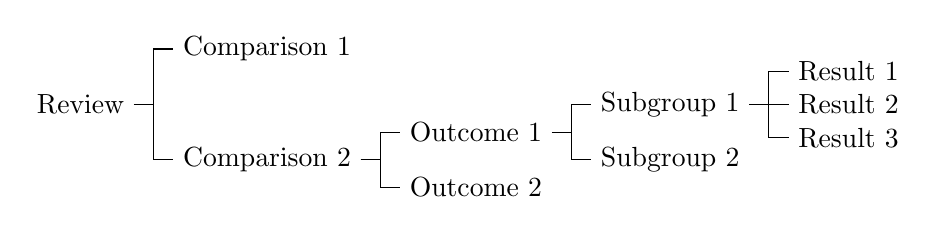
\begin{tikzpicture}
[grow = right, anchor = west,
  growth parent anchor=east, % added code
  parent anchor=east, level distance=.5cm,
  sibling distance=2em, level 1/.style={sibling distance=2em}, level 2/.style={sibling distance=2em},
  level 3/.style={sibling distance=2em}, level 4/.style={sibling distance=1.2em}]
  \node {Review} [edge from parent fork right]
    child { node {Comparison 2}
      child { node {Outcome 2}}
      child { node {Outcome 1}
        child { node {Subgroup 2}}
        child { node {Subgroup 1}
          child  { node {Result 3}}
          child  { node {Result 2}}
          child  { node {Result 1}}
          }}
    }
    child [missing] {}
    child { node {Comparison 1}};
\end{tikzpicture}
%\caption{Structure of a hypothetical review with two different comparisons\label{review.structure}}
\label{review.structure}
\end{figure}
\end{frame}





\begin{frame}[fragile]{Dataset Properties}
Review or study level:
% latex table generated in R 3.5.1 by xtable 1.8-3 package
% Mon May 20 22:21:48 2019
\begin{table}[ht]
\centering
\begingroup\footnotesize
\begin{tabular}{lrrrr}
  & 5\% quantile & median & mean & 95\% quantile \\ 
  \hline
Number of studies & 1 & 7 & 12 & 40 \\ 
   \hline
\hline
Number of comparisons & 1 & 2 & 4 & 12 \\ 
  Number of meta-analyses & 2 & 19 & 37 & 132 \\ 
   \hline
Study years & 1981 & 2002 & 2000 & 2013 \\ 
  Study sample size & 13 & 78 & 750 & 890 \\ 
  \end{tabular}
\endgroup
\end{table}

\end{frame}



\begin{frame}{Small Study Effects}
``The tendency for the smaller studies to show larger treatment effects'' \citep{Sterne}
\end{frame}


\begin{frame}{Small Study Effects}
Causes:
\begin{itemize}
\item Selective publication of studies with significant results - publication bias
\item Systematic differences in study settings
\end{itemize}
\end{frame}


\begin{frame}{Small Study Effect Tests}
Different approaches:
\begin{itemize}
\item Simple linear regression
\item Rank correlation
\end{itemize}

Special methods for binary outcomes	
\end{frame}


% \begin{frame}[fragile]{Small Study Effect Tests}
% Funnel plots (continuous outcome examples):
% 
% \vspace{-1.2cm}
% 
% <<message = FALSE, echo=FALSE, warning = FALSE, fig.height=4>>=
% par(las = 1, mfrow = c(1, 2))
% funnel(meta.example)
% funnel(meta.nexample)
% @
% 
% \end{frame}
% 
% 
% \begin{frame}[fragile]{Regression based Tests}
% Radial plots (continuous outcome examples):
% 
% \vspace{-1.1cm}
% 
% <<message = FALSE, echo=FALSE, warning = FALSE, fig.height=4>>=
% par(las = 1, mfrow = c(1,2))
% biased.rev$inv <- 1/biased.rev$se
% plot(y = (biased.rev$effect/biased.rev$se), x = (biased.rev$se^-1), xlim = c(0, 6), xlab = "inverse standard error", 
% 		 ylab = "mean diff. / std. error")
% 
% unbiased.rev$inv <- 1/unbiased.rev$se
% plot(y = (unbiased.rev$effect/unbiased.rev$se), x = (unbiased.rev$inv), xlim = c(0, 1.2), 
% 		 ylim = c(-18, 0), xlab = "inverse standard error", ylab = "mean diff. / std. error")
% @
% 
% \end{frame}


\begin{frame}{Regression based Tests}
study $i$ of $n$ studies, effects $\theta_i$ and variances $v_i$, s.e. $s_i$

$\theta_M$ is the pooled effect and $\tau^2$ the between-study variance.

Let $y_{i} = \theta_{i}/_{i}$ and $x_i = 1/s_i$
\begin{itemize}
\item \citet{Egger} : Simple linear regression \\ $y_i = \beta_0 + \beta_1 x_i, \epsilon_i \sim N(0, \sigma)$
\item \citet{thompson.sharp} : extension of Egger with study weights $v_{i} + \tau^2$ 
\end{itemize}

\end{frame}

\begin{frame}[fragile]{Egger's Test examples}
Test for non-zero intercept $\beta_{0}$

\vspace{-1.1cm}
\begin{knitrout}
\definecolor{shadecolor}{rgb}{0.969, 0.969, 0.969}\color{fgcolor}
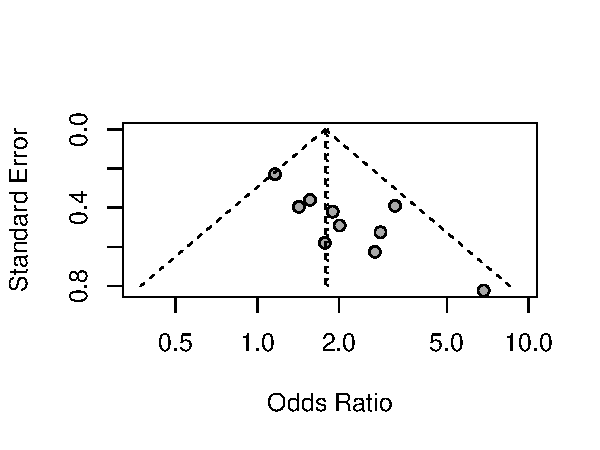
\includegraphics[width=\maxwidth]{figure/unnamed-chunk-4-1} 

\end{knitrout}
\end{frame}


\begin{frame}{Regression Tests for Binary Outcomes}

\begin{itemize}
\item \citet{Peters} :$x_i = 1/n_i$ instead $1/s_i$, inverse variances as weight.
\item \citet{Harbord} :$x_i$ = score of the log-likelihood of a proportion and inverse variances as weights.
\item \citet{Rucker} :Use arcsine variance stabilizing transformation for variances and effects, do e.g. Egger's test.
\end{itemize}
\end{frame}


\begin{frame}{Rank based tests}
\citet{begg.ties}: \\
Let $y_{i}$ be $\frac{\theta_i - \theta_M}{v_i}$ and $x_i$ its variance ($\neq v_i$)

$u$ the number of pairs $(y_{i}, x_{i})$ ranked in the same order, $l$
the number of pairs in the opposite order

$Z = \frac{(u - l)}{\sqrt{n(n-1)(2n + 5)/18}}$  is a test statistic
\end{frame}

\begin{frame}{Rank based tests}
\citet{Schwarzer}: \\
$e_t$ number of events in the treatment group

$E_t$ follows hypergeometric distribution: calculate $\mathbb{E}(E_{t})$ and variances

proceed as in \citet{begg.ties}
\end{frame}


\begin{frame}{Test Results}
Inclusion criteria (from \citet{Ioannidis2007}):
\begin{itemize}
\item $n \geq 10$
\item at least one statistically significant effect in a study
\item $\frac{\hat{v_{\textrm{max}}}^2}{\hat{v_{\textrm{min}}}^2} > 4$
\item $I^2 < 0.5$
\end{itemize}

From 5338 with $n \geq 10$, 1484 remain.
\end{frame}



\begin{frame}[fragile]{Continuous Outcome Test Results}
$p$-values distribution, $n$ = 294:

\vspace{-2mm}
\begin{knitrout}
\definecolor{shadecolor}{rgb}{0.969, 0.969, 0.969}\color{fgcolor}
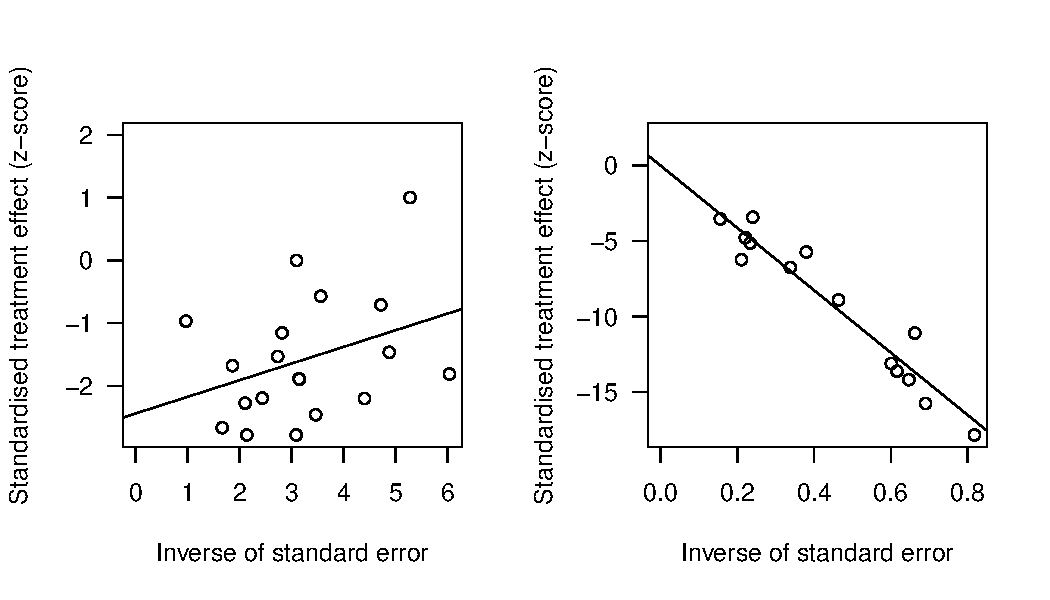
\includegraphics[width=\maxwidth]{figure/unnamed-chunk-5-1} 

\end{knitrout}
\end{frame}

\begin{frame}[fragile]{Binary Outcome Test Results}
$p$-values distribution, $n$ = 1190:

\vspace{-2mm}
\begin{knitrout}
\definecolor{shadecolor}{rgb}{0.969, 0.969, 0.969}\color{fgcolor}
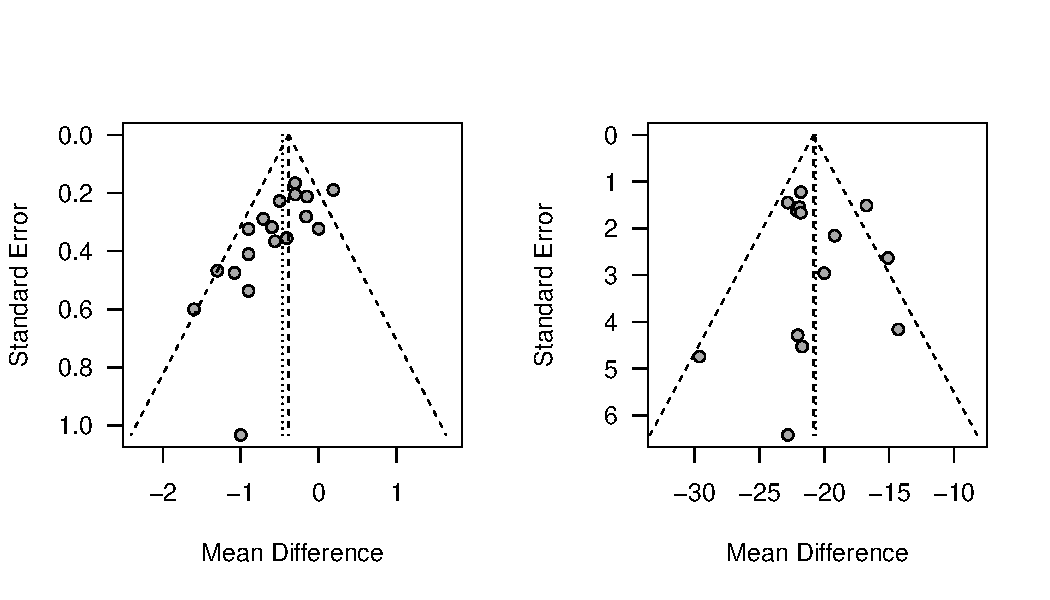
\includegraphics[width=\maxwidth]{figure/unnamed-chunk-6-1} 

\end{knitrout}
\end{frame}

\begin{frame}[fragile]{Agreement in significance}
Number of significant test results per meta-analysis:

\vspace{-2mm}
\begin{knitrout}
\definecolor{shadecolor}{rgb}{0.969, 0.969, 0.969}\color{fgcolor}
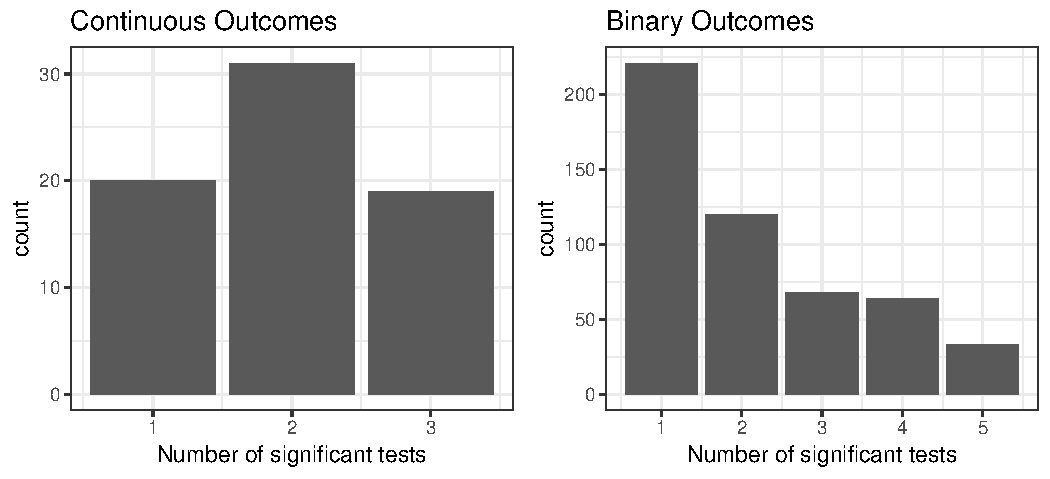
\includegraphics[width=\maxwidth]{figure/unnamed-chunk-7-1} 

\end{knitrout}
\end{frame}

\begin{frame}{Small Study Effect Adjustment}
Three methods:
\begin{itemize}
\item Regression
\item Copas selection model
\item Trim-and-fill
\end{itemize}
\end{frame}

\begin{frame}{Adjustment by regression}
$y_i = \theta_i/s_i, x_i = 1/s_i$

$y_i = \beta_0 + \beta_1 x_i, \epsilon_i \sim N(0, \sigma)$

$\beta_1$ is the weighted mean treatment effect if $\beta_0 = 0$
\end{frame}


\begin{frame}{Adjustment by regression}
Radial plots (continuous outcome examples):

\vspace{-1.1cm}

\begin{knitrout}
\definecolor{shadecolor}{rgb}{0.969, 0.969, 0.969}\color{fgcolor}
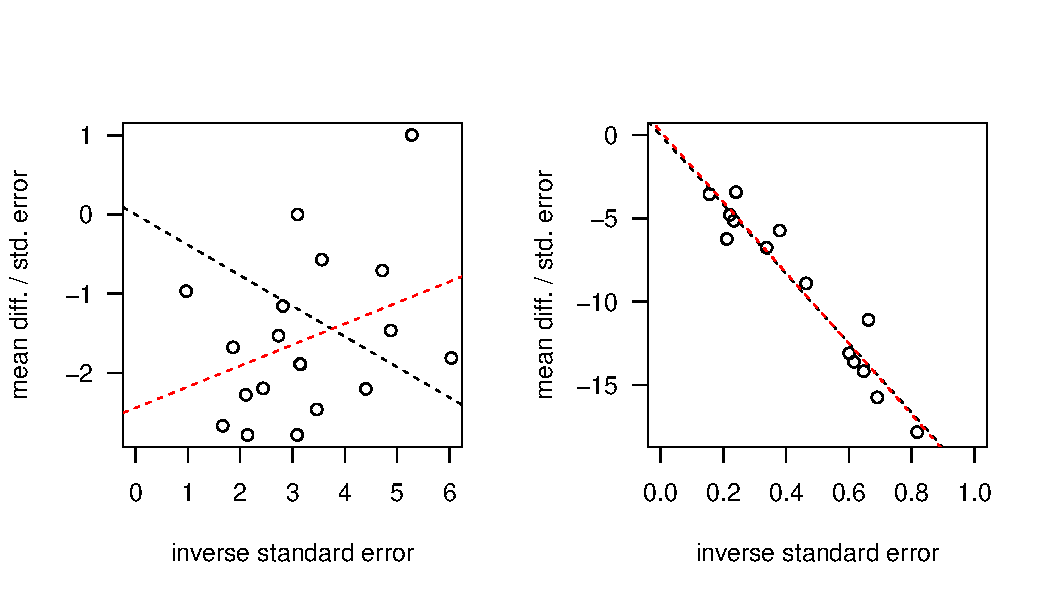
\includegraphics[width=\maxwidth]{figure/unnamed-chunk-8-1} 

\end{knitrout}
\end{frame}



\begin{frame}[fragile]{Limit Meta-Analysis}
Extended random effects model:

\vspace{-4mm}
\begin{align}
\theta_i = \beta_0 + \beta_1(\sqrt{v_i + \tau^2}) + \epsilon_i(\sqrt{v_i + \tau^2}), \nonumber \\
\epsilon_{i} \stackrel{\textrm{iid}}{\sim} N(0,1) \nonumber
\end{align}

Use $\mathbb{E}(y_{i}) \rightarrow \beta_{0} + \beta_{1}\tau$ for $\sqrt{v_{i}} \rightarrow 0$
as corrected treatment efffect.
\end{frame}



\begin{frame}[fragile]{Limit Meta-Analysis}
Funnel plot with effect with infinite precision:

\vspace{-1.1cm}
\begin{knitrout}
\definecolor{shadecolor}{rgb}{0.969, 0.969, 0.969}\color{fgcolor}
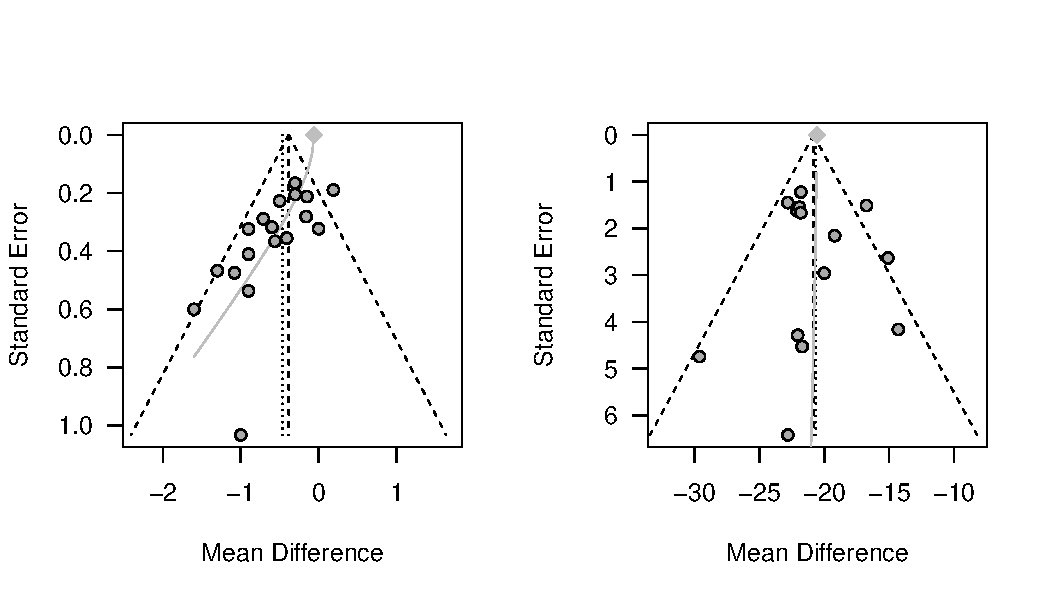
\includegraphics[width=\maxwidth]{figure/unnamed-chunk-9-1} 

\end{knitrout}
\end{frame}



\begin{frame}{Selection model}
\citet{Copas1}: model based on a bivariate normal distribution:

\vspace{-8mm}
\begin{align}
\hat{theta_i} = \theta_{i} + v_i\epsilon_i \label{population.model2} \\
\theta_i \sim N(\theta, \tau^2) \label{population.model} \\
z_i = a + b/s_i + \delta_i \label{selection.model}
\end{align}

\ref{population.model}, \ref{population.model2} is called population model, \ref{selection.model} the selection model

$(\epsilon_i, \delta_i)$ are standard normal residuals with correlation $\rho = cor(y_i, z_i)$.
\end{frame}


\begin{frame}[fragile]{Sensitivity Analysis}
Model the selection process with different $a,b$

Test if small study effect is significant, by including \\ $\theta_i = \theta_i + \beta s_i + v_{i}\epsilon_i$

Estimation: Select $a, b$ such that $H0$ can not be rejected and estimated
number of unpublished studies is minimal.
\end{frame}


\begin{frame}{Trim-and-Fill}
Mirror studies that cause asymmetry:
\vspace{-1.2cm}

\begin{knitrout}
\definecolor{shadecolor}{rgb}{0.969, 0.969, 0.969}\color{fgcolor}
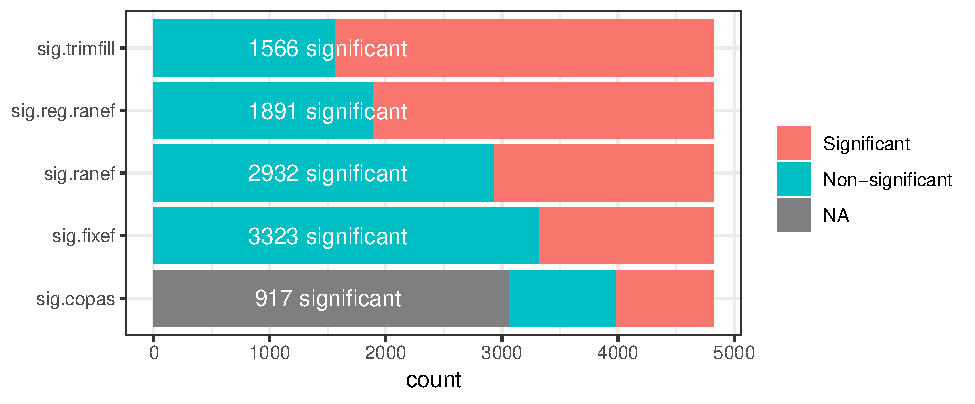
\includegraphics[width=\maxwidth]{figure/unnamed-chunk-10-1} 

\end{knitrout}
\end{frame}


\begin{frame}[fragile]{Results:}
Difference between random and fixed effects meta-analysis estimate: $|\theta_f - \theta_{r}|$

\vspace{-3mm}
\begin{knitrout}
\definecolor{shadecolor}{rgb}{0.969, 0.969, 0.969}\color{fgcolor}
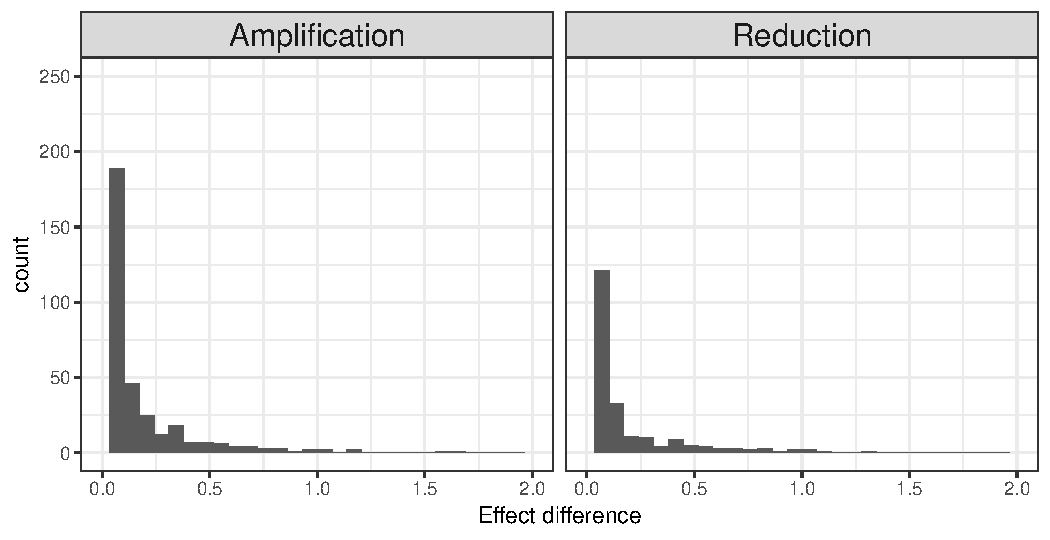
\includegraphics[width=\maxwidth]{figure/unnamed-chunk-11-1} 

\end{knitrout}
\end{frame}


\begin{frame}[fragile]{Adjustment Results: Trim-and-fill}
Absolute difference between adjusted and fixed effects meta-analysis estimate: $|{\theta_f} - {\theta_{\textrm{adjusted}}}|$

\vspace{-3mm}
\begin{knitrout}
\definecolor{shadecolor}{rgb}{0.969, 0.969, 0.969}\color{fgcolor}
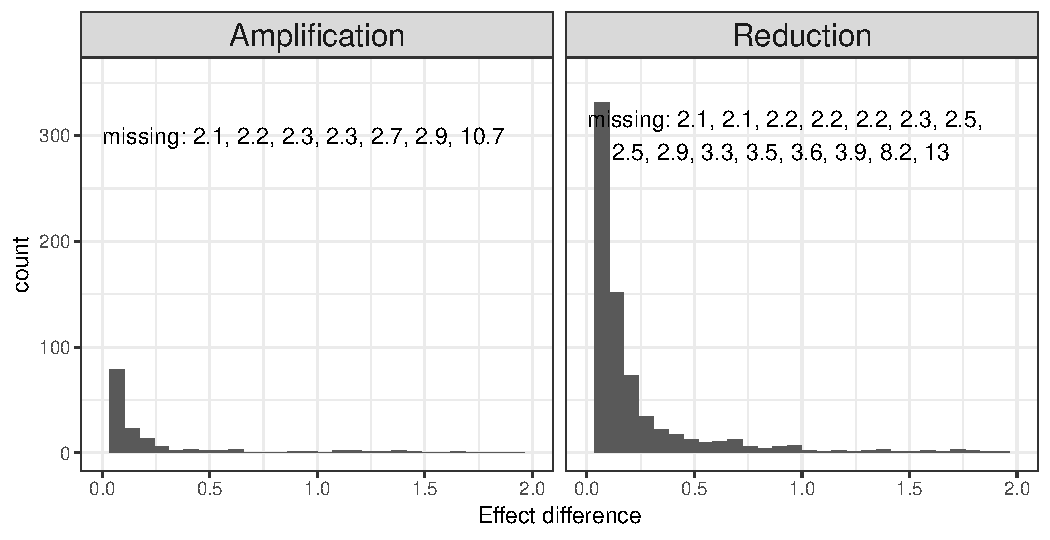
\includegraphics[width=\maxwidth]{figure/unnamed-chunk-12-1} 

\end{knitrout}
\end{frame}


\begin{frame}[fragile]{Adjustment Results: Copas}
Absolute difference between adjusted and fixed effects meta-analysis estimate: $|{\theta_f} - {\theta_{\textrm{adjusted}}}|$

\vspace{-3mm}
\begin{knitrout}
\definecolor{shadecolor}{rgb}{0.969, 0.969, 0.969}\color{fgcolor}
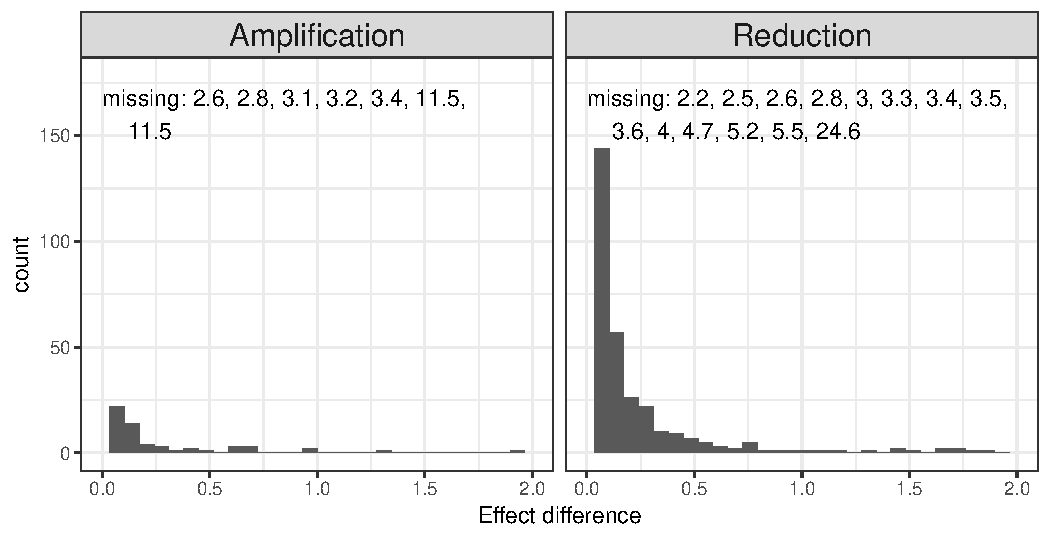
\includegraphics[width=\maxwidth]{figure/unnamed-chunk-13-1} 

\end{knitrout}
\end{frame}


\begin{frame}[fragile]{Adjustment Results: Regression}
Absolute difference between adjusted and fixed effects meta-analysis estimate: $|{\theta_f} - {\theta_{\textrm{adjusted}}}|$

\vspace{-3mm}
\begin{knitrout}
\definecolor{shadecolor}{rgb}{0.969, 0.969, 0.969}\color{fgcolor}
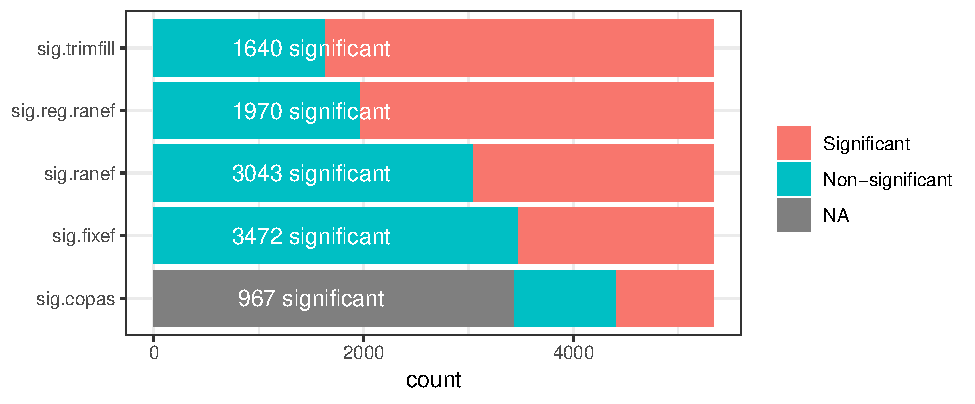
\includegraphics[width=\maxwidth]{figure/unnamed-chunk-14-1} 

\end{knitrout}
\end{frame}


\begin{frame}[fragile]{Results:}
Random and fixed effects meta-analyses test statistics:

\vspace{-3mm} 
\begin{knitrout}
\definecolor{shadecolor}{rgb}{0.969, 0.969, 0.969}\color{fgcolor}
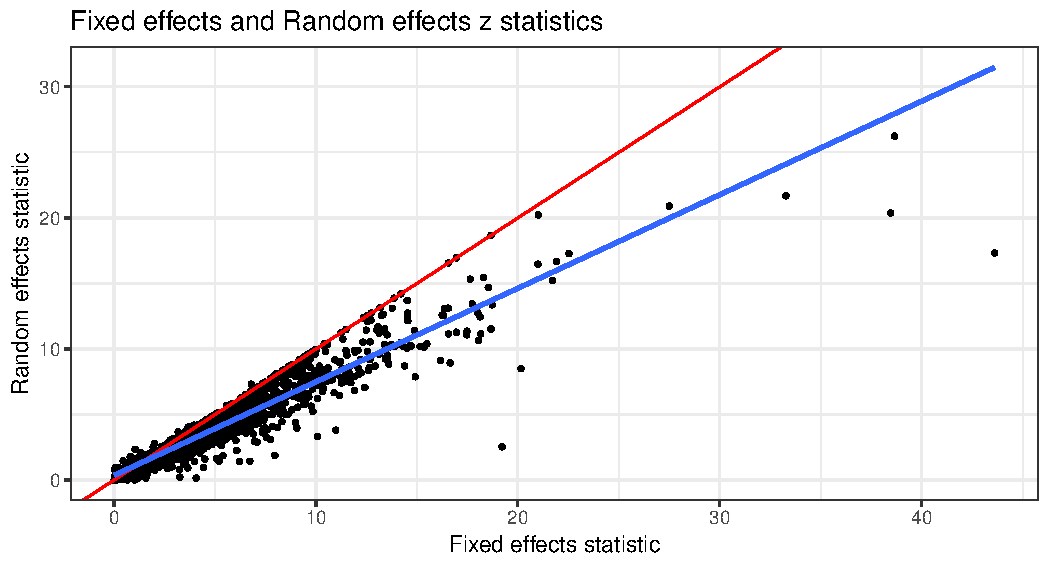
\includegraphics[width=\maxwidth]{figure/unnamed-chunk-15-1} 

\end{knitrout}
\end{frame}


\begin{frame}[fragile]{Adjustment Results: Trim-and-fill}
Adjusted and meta-analysis test statistics:

\vspace{-3mm} 
\begin{knitrout}
\definecolor{shadecolor}{rgb}{0.969, 0.969, 0.969}\color{fgcolor}
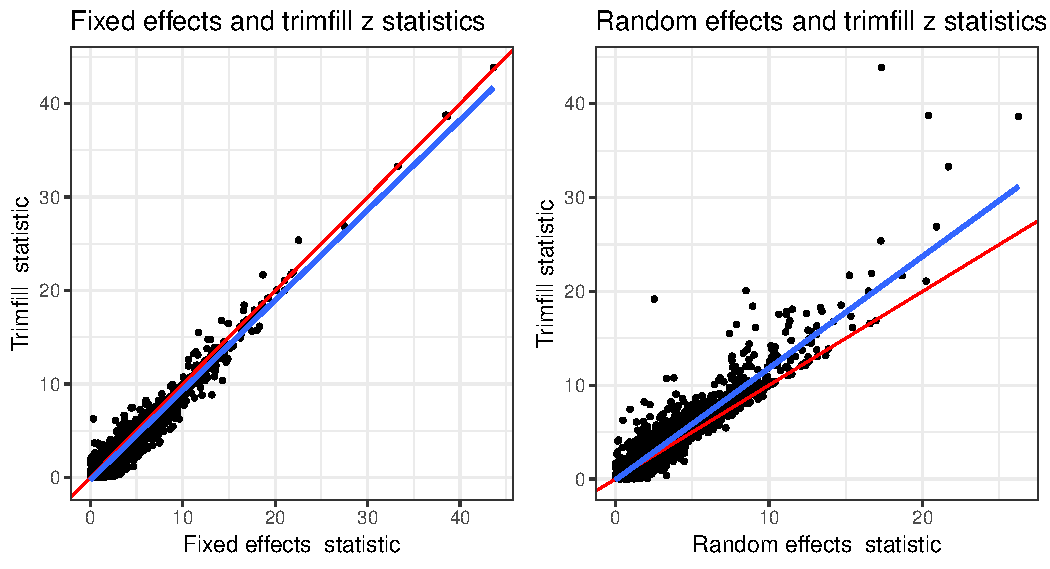
\includegraphics[width=\maxwidth]{figure/unnamed-chunk-16-1} 

\end{knitrout}
\end{frame}


\begin{frame}[fragile]{Adjustment Results: Copas}
Adjusted and meta-analysis test statistics:

\vspace{-3mm}
\begin{knitrout}
\definecolor{shadecolor}{rgb}{0.969, 0.969, 0.969}\color{fgcolor}
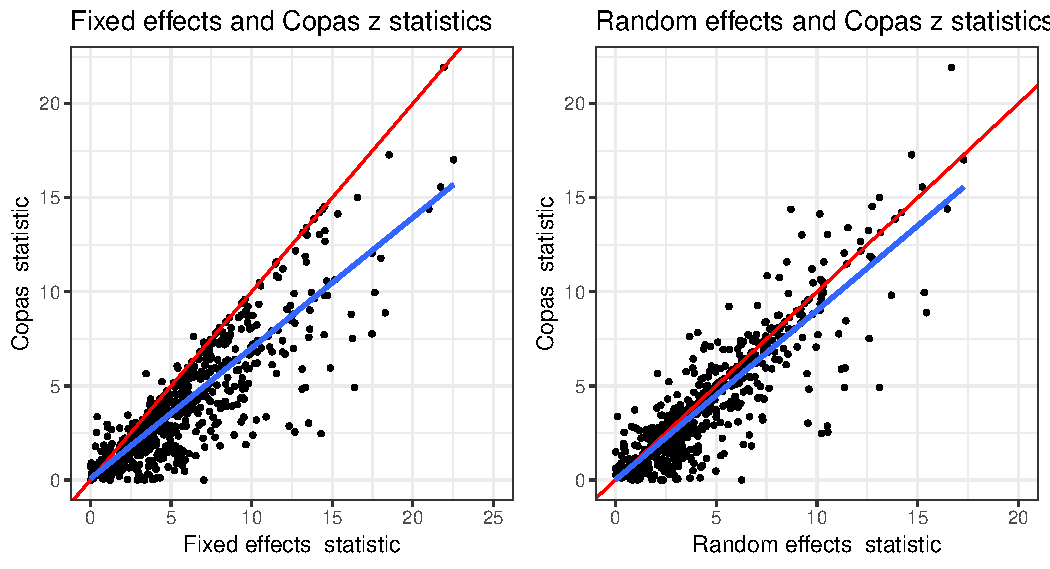
\includegraphics[width=\maxwidth]{figure/unnamed-chunk-17-1} 

\end{knitrout}
\end{frame}


\begin{frame}[fragile]{Adjustment Results: Regression}
Adjusted and meta-analysis test statistics:

\vspace{-3mm}
\begin{knitrout}
\definecolor{shadecolor}{rgb}{0.969, 0.969, 0.969}\color{fgcolor}
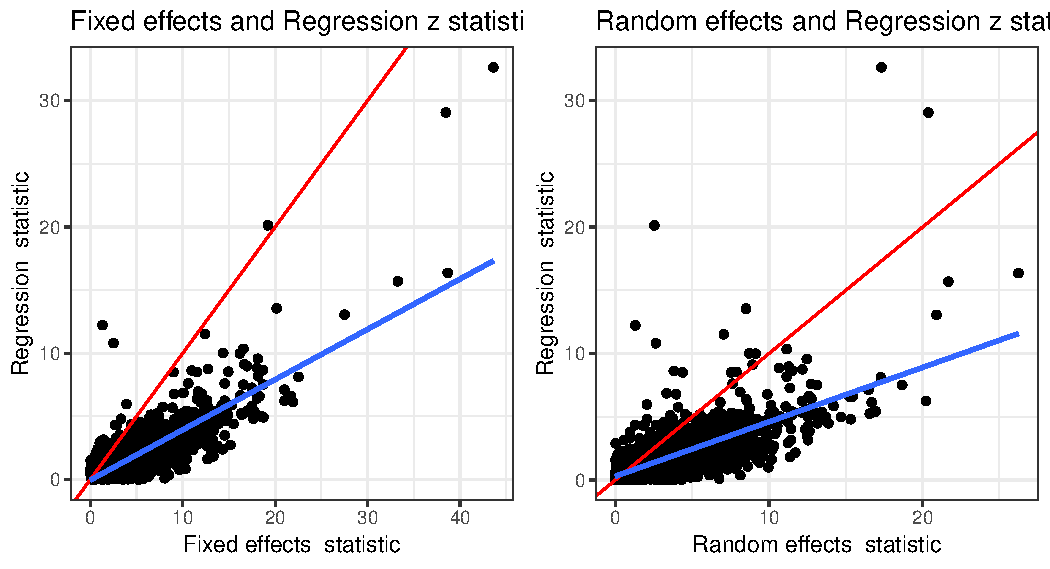
\includegraphics[width=\maxwidth]{figure/unnamed-chunk-18-1} 

\end{knitrout}
\end{frame}


\begin{frame}[fragile]{Adjustment Results}
Missing study proportions:

\vspace{-3mm}
\begin{knitrout}
\definecolor{shadecolor}{rgb}{0.969, 0.969, 0.969}\color{fgcolor}
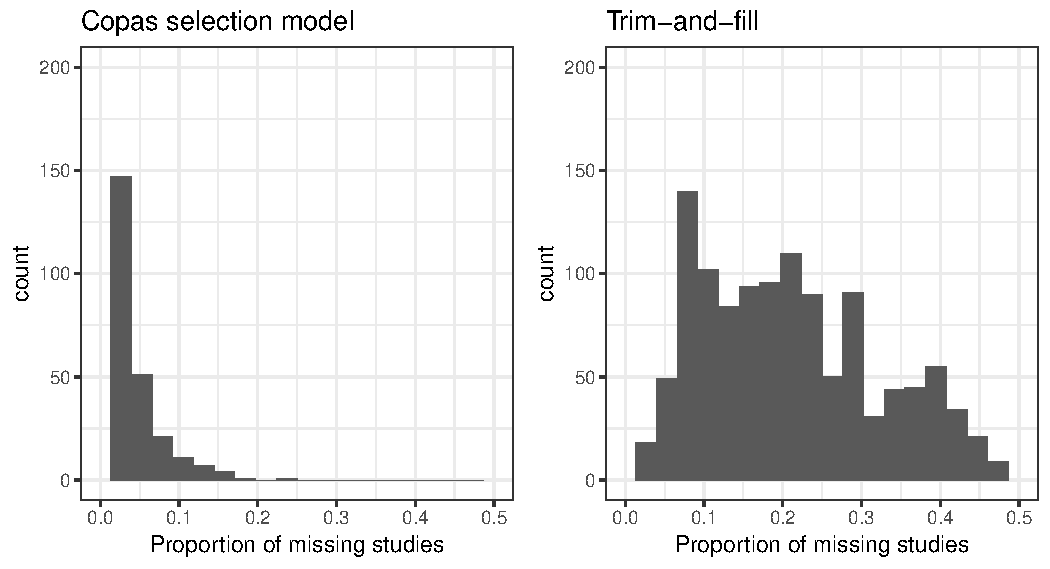
\includegraphics[width=\maxwidth]{figure/unnamed-chunk-19-1} 

\end{knitrout}
\end{frame}

\begin{frame}[fragile]{Extreme Results}
RR reduction by trimfill (-3.9), side effects

\begin{knitrout}
\definecolor{shadecolor}{rgb}{0.969, 0.969, 0.969}\color{fgcolor}
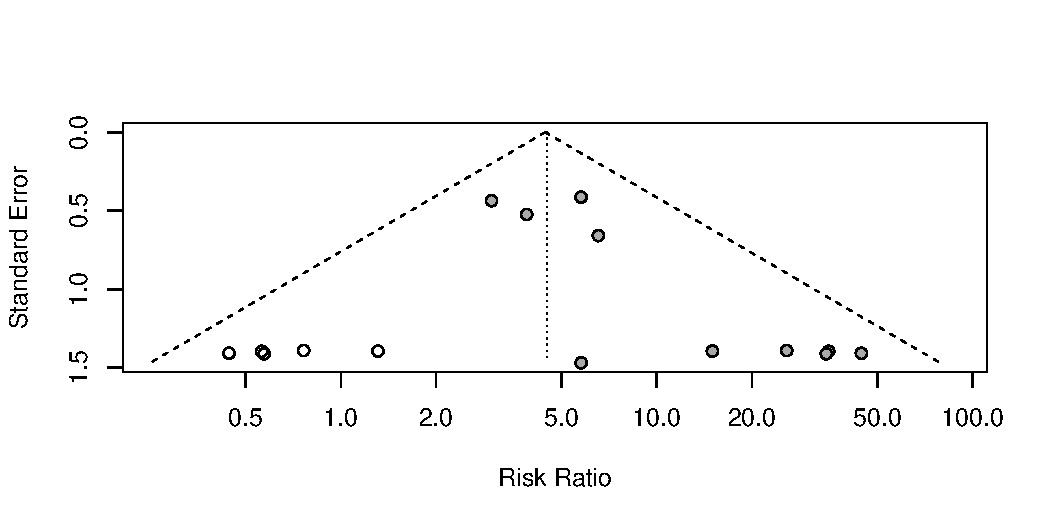
\includegraphics[width=\maxwidth]{figure/unnamed-chunk-20-1} 

\end{knitrout}
\end{frame}

\begin{frame}[fragile]{Extreme Results}
RR Reduction by copas selection model (-4), pain relief

\begin{knitrout}
\definecolor{shadecolor}{rgb}{0.969, 0.969, 0.969}\color{fgcolor}
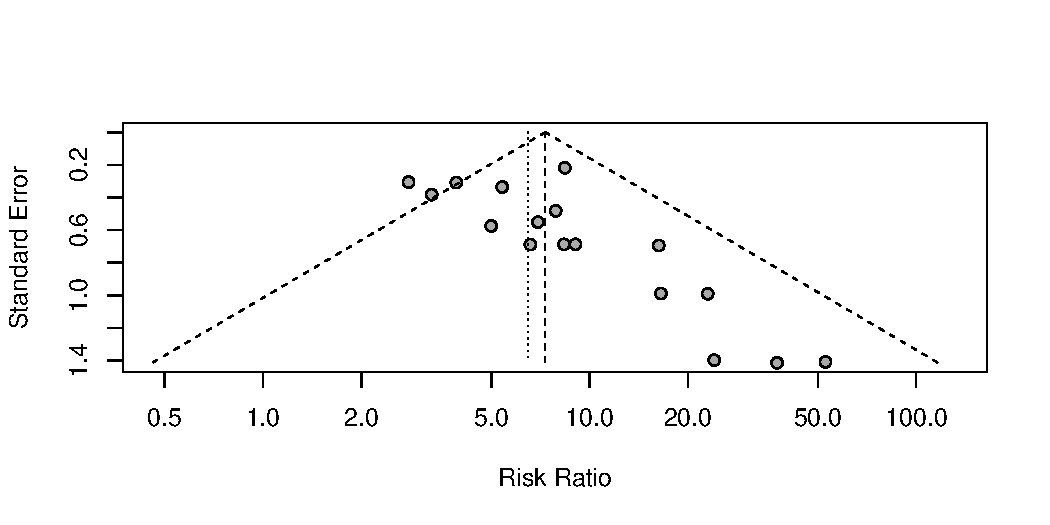
\includegraphics[width=\maxwidth]{figure/unnamed-chunk-21-1} 

\end{knitrout}
\end{frame}

\begin{frame}[fragile]{Extreme Results}
RR Amplification by regression (+14), side effects

\begin{knitrout}
\definecolor{shadecolor}{rgb}{0.969, 0.969, 0.969}\color{fgcolor}
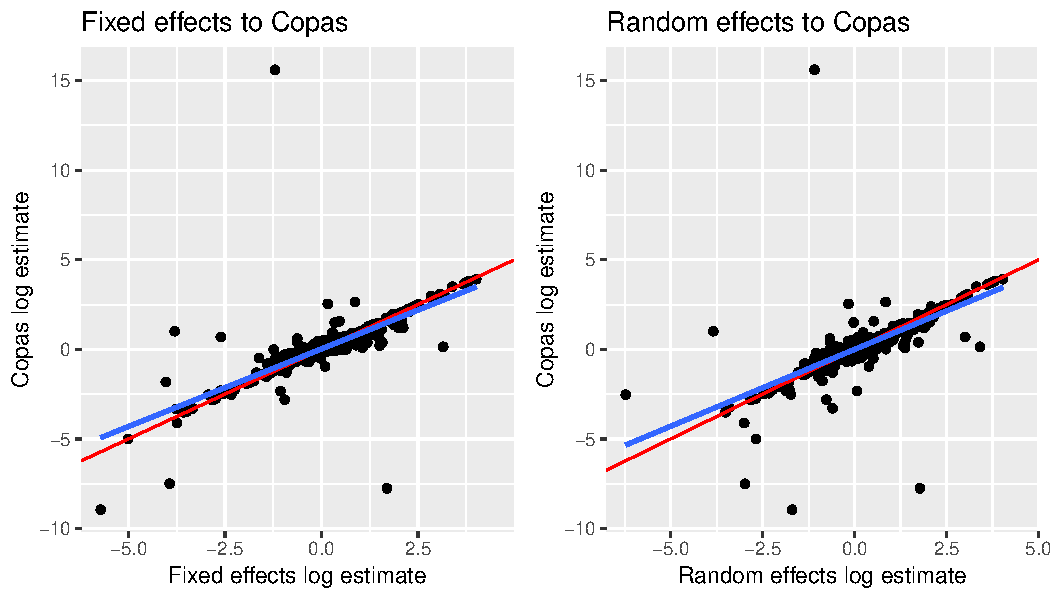
\includegraphics[width=\maxwidth]{figure/unnamed-chunk-22-1} 

\end{knitrout}
\end{frame}

\begin{frame}[fragile]{Discussion}
\begin{itemize}
\item Proportion of positive tests is well above 10\%
\item Effect sizes and evidence for treatment effect is diminishued
\item Limitations: not only primary outcomes, adjustment methods known to
perform poorly under the 0
\end{itemize}
\end{frame}


\begin{frame}[fragile]{Outlook}
\begin{itemize}
\item Connect results with different medical fields, look for differences
\item Connect results with single studies and journals (?)
\end{itemize}
\end{frame}













%%%%%%%%%%%%%%%%%%%%%%%%%%%%%%%%%%%%%%%%%%%%%%%%%%%%%%%%%%%%%%%%%%%%%%%%
%Backup Slides%%%%%%%%%%%%%%%%%%%%%%%%%%%%%%%%%%%%%%%%%%%%%%%%%%%%%%%%%%
%%%%%%%%%%%%%%%%%%%%%%%%%%%%%%%%%%%%%%%%%%%%%%%%%%%%%%%%%%%%%%%%%%%%%%%%

\begin{frame}[fragile]{Adjustment Results: Trim-and-fill}
Treatment effect difference:

\vspace{-3mm}
\begin{knitrout}
\definecolor{shadecolor}{rgb}{0.969, 0.969, 0.969}\color{fgcolor}
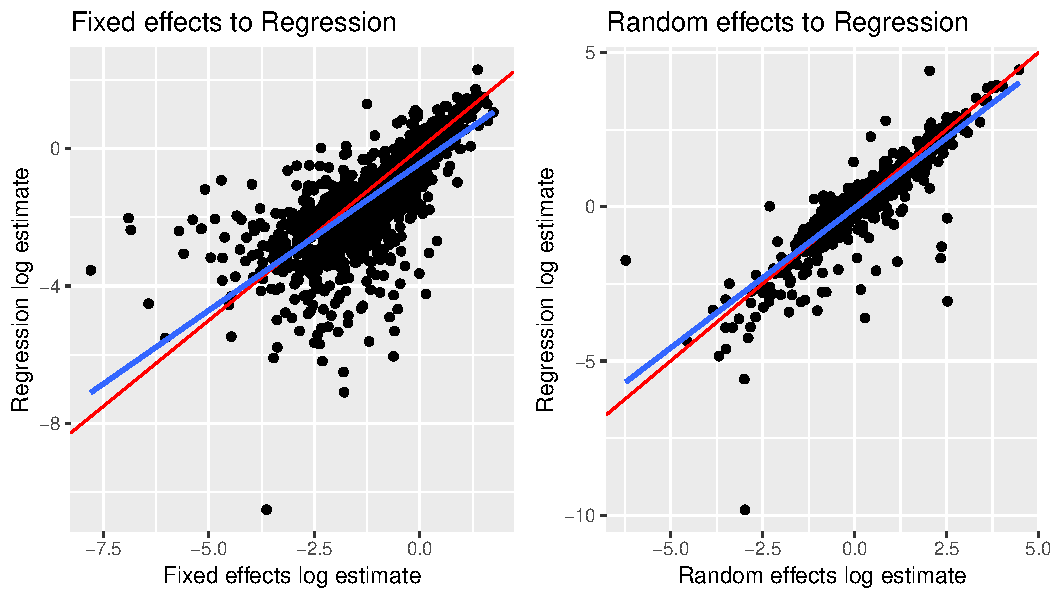
\includegraphics[width=\maxwidth]{figure/unnamed-chunk-23-1} 

\end{knitrout}
\end{frame}


\begin{frame}[fragile]{Adjustment Results: Copas}
Treatment effect difference:

\vspace{-3mm}
\begin{knitrout}
\definecolor{shadecolor}{rgb}{0.969, 0.969, 0.969}\color{fgcolor}
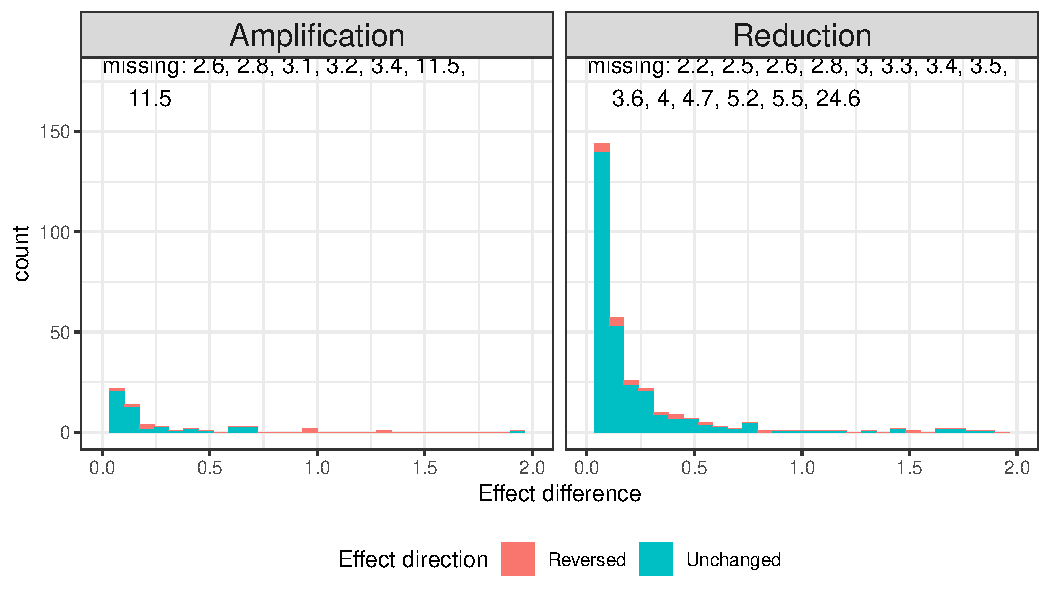
\includegraphics[width=\maxwidth]{figure/unnamed-chunk-24-1} 

\end{knitrout}
\end{frame}


\begin{frame}[fragile]{Adjustment Results: Regression}
Treatment effect difference:

\vspace{-3mm}
\begin{knitrout}
\definecolor{shadecolor}{rgb}{0.969, 0.969, 0.969}\color{fgcolor}
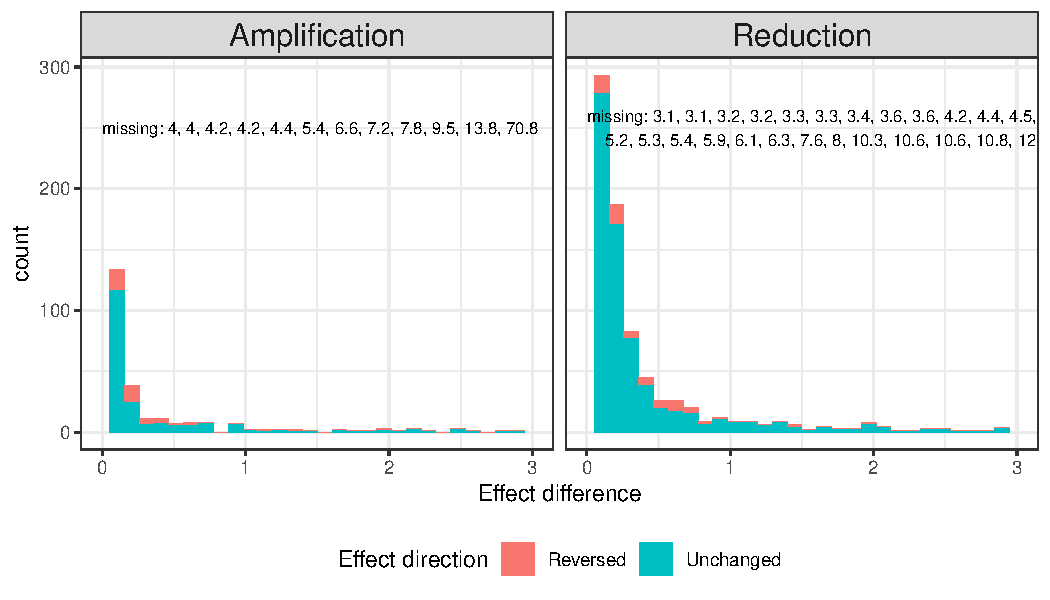
\includegraphics[width=\maxwidth]{figure/unnamed-chunk-25-1} 

\end{knitrout}
\end{frame}

\begin{frame}[fragile]{Results}
log treatment effect estimates:

\vspace{-3mm}
\begin{knitrout}
\definecolor{shadecolor}{rgb}{0.969, 0.969, 0.969}\color{fgcolor}
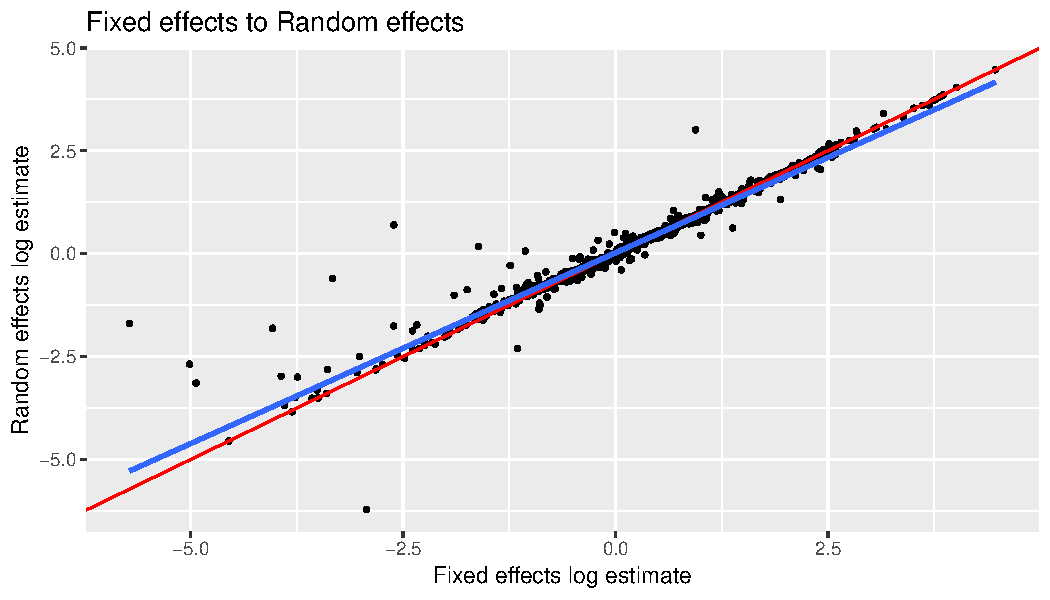
\includegraphics[width=\maxwidth]{figure/unnamed-chunk-26-1} 

\end{knitrout}
\end{frame}

\begin{frame}[fragile]{Adjustment Results: Trim-and-fill}
log treatment effect estimates:

\vspace{-3mm}
\begin{knitrout}
\definecolor{shadecolor}{rgb}{0.969, 0.969, 0.969}\color{fgcolor}
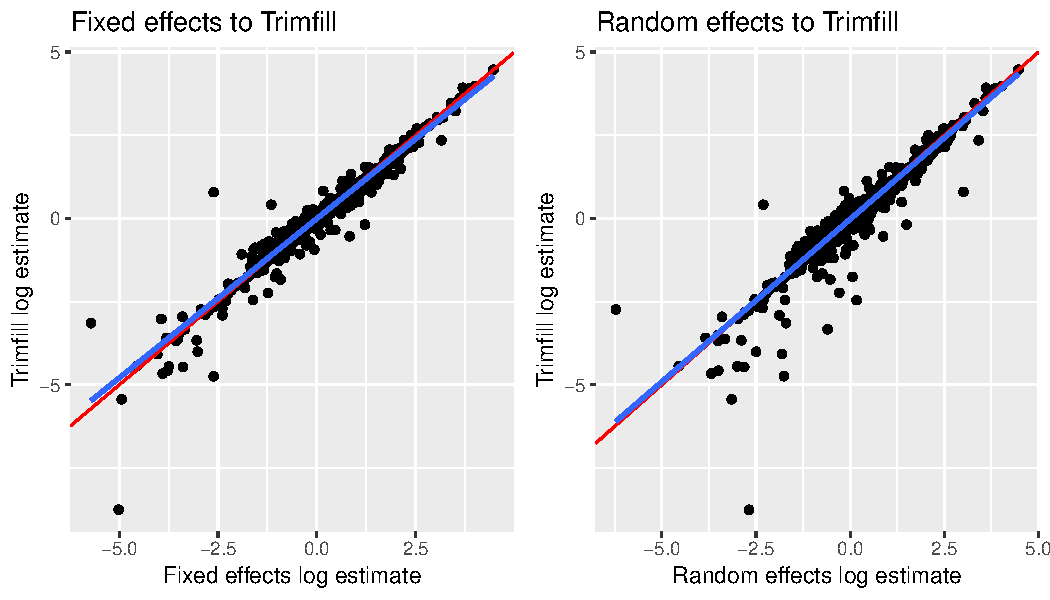
\includegraphics[width=\maxwidth]{figure/unnamed-chunk-27-1} 

\end{knitrout}
\end{frame}


\begin{frame}[fragile]{Adjustment Results: Copas}
log treatment effect estimates:

\vspace{-3mm}
\begin{knitrout}
\definecolor{shadecolor}{rgb}{0.969, 0.969, 0.969}\color{fgcolor}
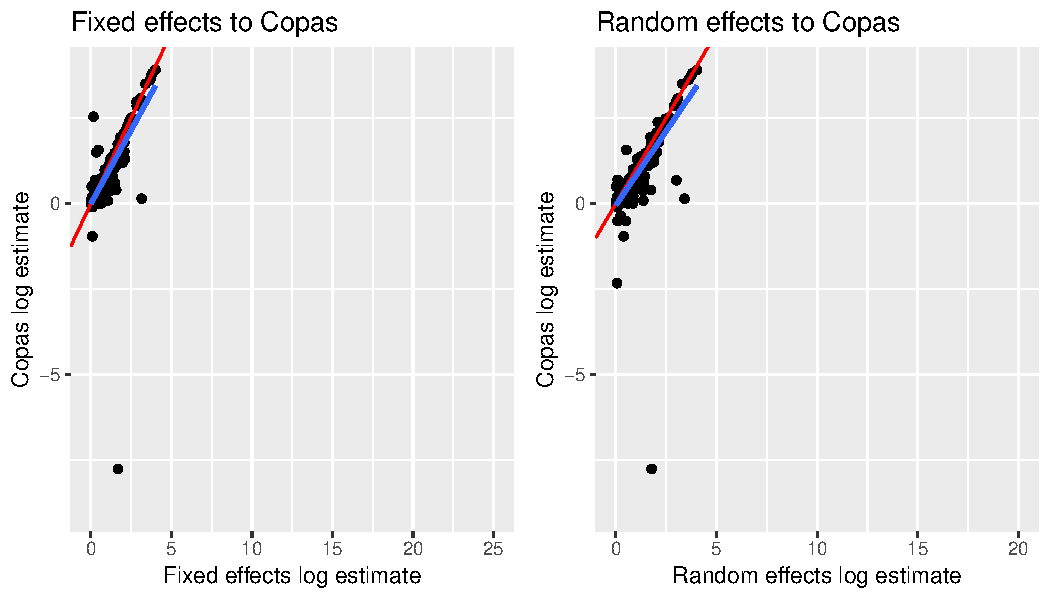
\includegraphics[width=\maxwidth]{figure/unnamed-chunk-28-1} 

\end{knitrout}
\end{frame}


\begin{frame}[fragile]{Adjustment Results: Regression}
log treatment effect estimates:

\vspace{-3mm}
\begin{knitrout}
\definecolor{shadecolor}{rgb}{0.969, 0.969, 0.969}\color{fgcolor}
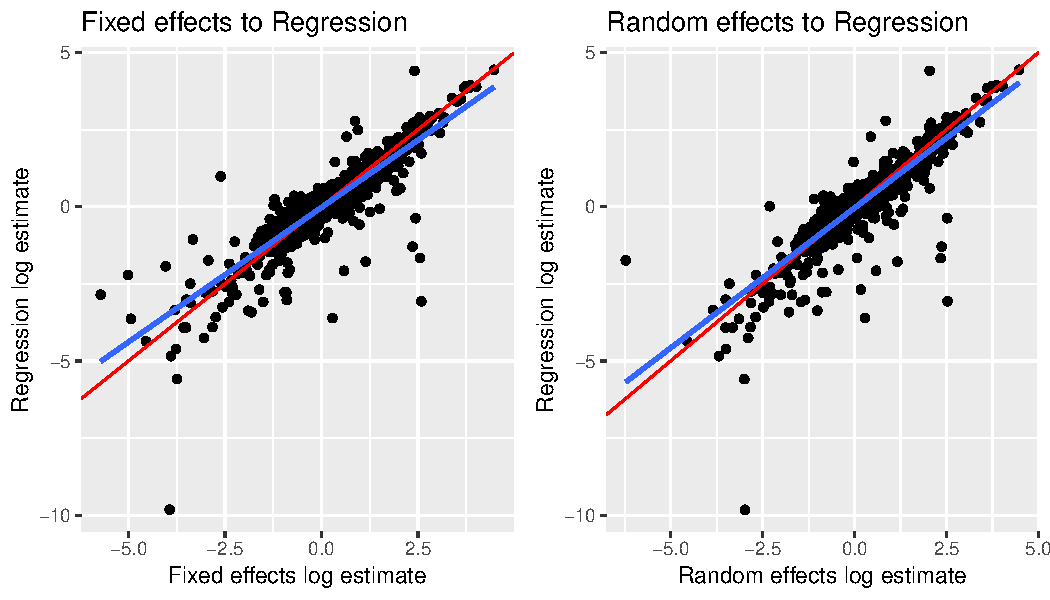
\includegraphics[width=\maxwidth]{figure/unnamed-chunk-29-1} 

\end{knitrout}
\end{frame}





\begin{frame}{References}
  \small
  \bibliographystyle{apalike}
\bibliography{illustration}
\end{frame}



%\appendix
%% Possible backup slides...

%% chapter division is accomplished with:
%% \part{Appendix}

% \begin{frame}[fragile]{Test Results: Significance}
% 
% <<echo = FALSE, fig.height = 4>>=
% grid.arrange(p.bin, p.cont, ncol = 2)
% @
% \end{frame}

% \begin{frame}[fragile]{Pooling Studies - Meta-Analysis}
% Multiple results in a meta-analysis group can be pooled:
% <<echo=FALSE, results = 'asis'>>=
% print(xtable(cum.repr.trials.subg, label = "repr.groups", align = "lrrr", digits = 0), include.rownames = F, size = "footnotesize")
% @
% \end{frame}

% \begin{frame}{Dataset Structure}
% \begin{itemize}
% \item Comparison: What is compared, e.g. treatment vs. control
% \item Outcome: How it is compared
% \item Subgroup: Subgroup affiliation
% \item Meta-Analysis Group: Results from same comparison, outcome and subgroup
% \end{itemize}
% \end{frame}

% \begin{frame}[fragile]{Dataset Properties}
% Missing data:
% <<echo=FALSE, results = 'asis'>>=
% print(xtable(missing.table, align = "lr"), include.rownames = T, include.colnames = F)
% @
% \end{frame}




% \begin{frame}{Adjustment by regression}
% Similar to the tests, but with unnormalized effect $y_{i}$:
% 
% \begin{align}
% y_{i} = \beta_{0} + \beta_{1}x_{i}
% \end{align}
% 
% $\beta_{0}$	 corresponds to $y_{i}$ with $x_{i} = 0$
% \end{frame}
% 
% \begin{frame}[fragile]{Adjustment by regression}
% Linear regression method:
% 
% <<echo = FALSE, fig.height = 3>>=
% grid.arrange(reg.1, reg.2, ncol = 2)
% @
% \end{frame}


% \begin{frame}[fragile]{Thompson and Sharp's Tests}
% Generalised radial plot with new standard error $x_i = s_i + \tau$
% 
% \vspace{-1.1cm}
% <<message = FALSE, echo=FALSE, warning = FALSE, fig.height= 4>>=
% par(las = 1, mfrow = c(1,2))
% tau.ex <- meta.example$tau
% biased.rev$inv <- 1/sqrt((biased.rev$se^2 + tau.ex^2))
% m.ex <- lm(formula = (biased.rev$effect*biased.rev$inv) ~ (biased.rev$inv), weights = biased.rev$se)
% biased.rev$inv <- 1/biased.rev$se
% plot(y = (biased.rev$effect/biased.rev$se), x = (biased.rev$inv), xlim = c(0, 4), xlab = "inverse standard error", 
% 		 ylab = "mean diff. / std. error")
% abline(coef = coef(m.ex), lty = 2, col = 2)
% 
% tau.nex <- meta.nexample$tau
% unbiased.rev$inv <- 1/sqrt((unbiased.rev$se^2 + tau.nex^2))
% m.nex <- lm(formula = (unbiased.rev$effect*unbiased.rev$inv) ~ (unbiased.rev$inv), weights = unbiased.rev$se)
% plot(y = (unbiased.rev$effect/unbiased.rev$se), x = (unbiased.rev$inv), xlim = c(0, .6), 
% 		 ylim = c(-18, 0), xlab = "inverse standard error", ylab = "mean diff. / std. error")
% abline(coef = coef(m.nex), lty = 2, col = 2)
% @
% 
% \end{frame}
% 
% 
% \begin{frame}[fragile]{Limit Meta-Analysis}
% \begin{align}
% y_{M,i} &= \beta_{0} + \beta_{1}(\sqrt{v_{i}/M + \tau^2}) + \epsilon_{i}(\sqrt{s_{i}/M + \tau^2}) \nonumber
% \end{align}
% 
% Letting $M \rightarrow \infty$ and substituting for all parameters and the observed residual
% 
% \vspace{-8mm}
% \begin{align}
% y_{\infty,i} &= \beta_{0} + \sqrt{\frac{\tau^2}{v_{i} + \tau^2}}(y_i - \beta_0)
% \end{align}
% \end{frame}
% 
% \begin{frame}[fragile]{Limit Meta-Analysis}
% By plugging in $s_i$ for $v_i$, $\hat{tau}$ for $\tau$ and $\hat{\beta_0}$, get new study effects:
% 
% Three different treatment effect estimates:
% \begin{itemize}
% \item Expectated adjusted treatment effect with infinite precision: $\hat{\beta_{0}^\star} + \hat{\beta_{1}}\hat{\tau}$
% \item Fixed effect estimate based on $(y_{\infty,1},.. , y_{\infty,n}$
% \item Slope $\beta_{\textrm{lim}}$ of best-fitting regression line in radial plot with $(y_{\infty,i}, s_{i})$
% \end{itemize}
% \end{frame}

\end{document}
